\documentclass[dvipdfmx,12pt]{beamer}

\usepackage{bxdpx-beamer}
\usepackage{pxjahyper}
\usepackage{minijs}
\usetheme{Annarbor}
\usepackage{mathpazo}
\usepackage{amsmath,amssymb}
\usepackage{graphicx}
\usepackage{array}

\title{Reference Point \\ for the Baseball Players in Japan}
\subtitle{Is the contribution of SABR metrics taken into account?}
\author{Reio TANJI}
\date{June.28,2018}
\institute{Osaka University}

\begin{document}
\begin{frame}\frametitle{Introduction}
\titlepage
\end{frame}

\section{Introduction}
\begin{frame}\frametitle{References}
 
 \begin{itemize}
  
  \item Pope \& Simonsohn (2011,Association for Phychological Science)
   
  ``Round Numbers as Goals : Evidence From Baseball, SAT Takers, and the Lab''
   
  \item Hakes \& Sauer (2006, Jornal of Economic Perspectives)
   
  ``An Economic Evaluation of the \textit{Moneyball} Hypothesis''
   
  \end{itemize}
 
\end{frame}

\begin{frame}\frametitle{Pope \& Simonsohn}

\begin{itemize}

\item Verify that \textbf{round numbers} in performance scales act as \textbf{reference points}, by examing three practical studies.

\item In the first study, they found that baseball players in MLB prefer finising the season with a batting average(AVG) just above .300, to that with just below .300.

\item Data : MLB player's play-by-play data from 1975 to 2008.

Players with at least 200 at bat (打数) : N=8,817

\end{itemize}

\end{frame}

\begin{frame}
\begin{center}

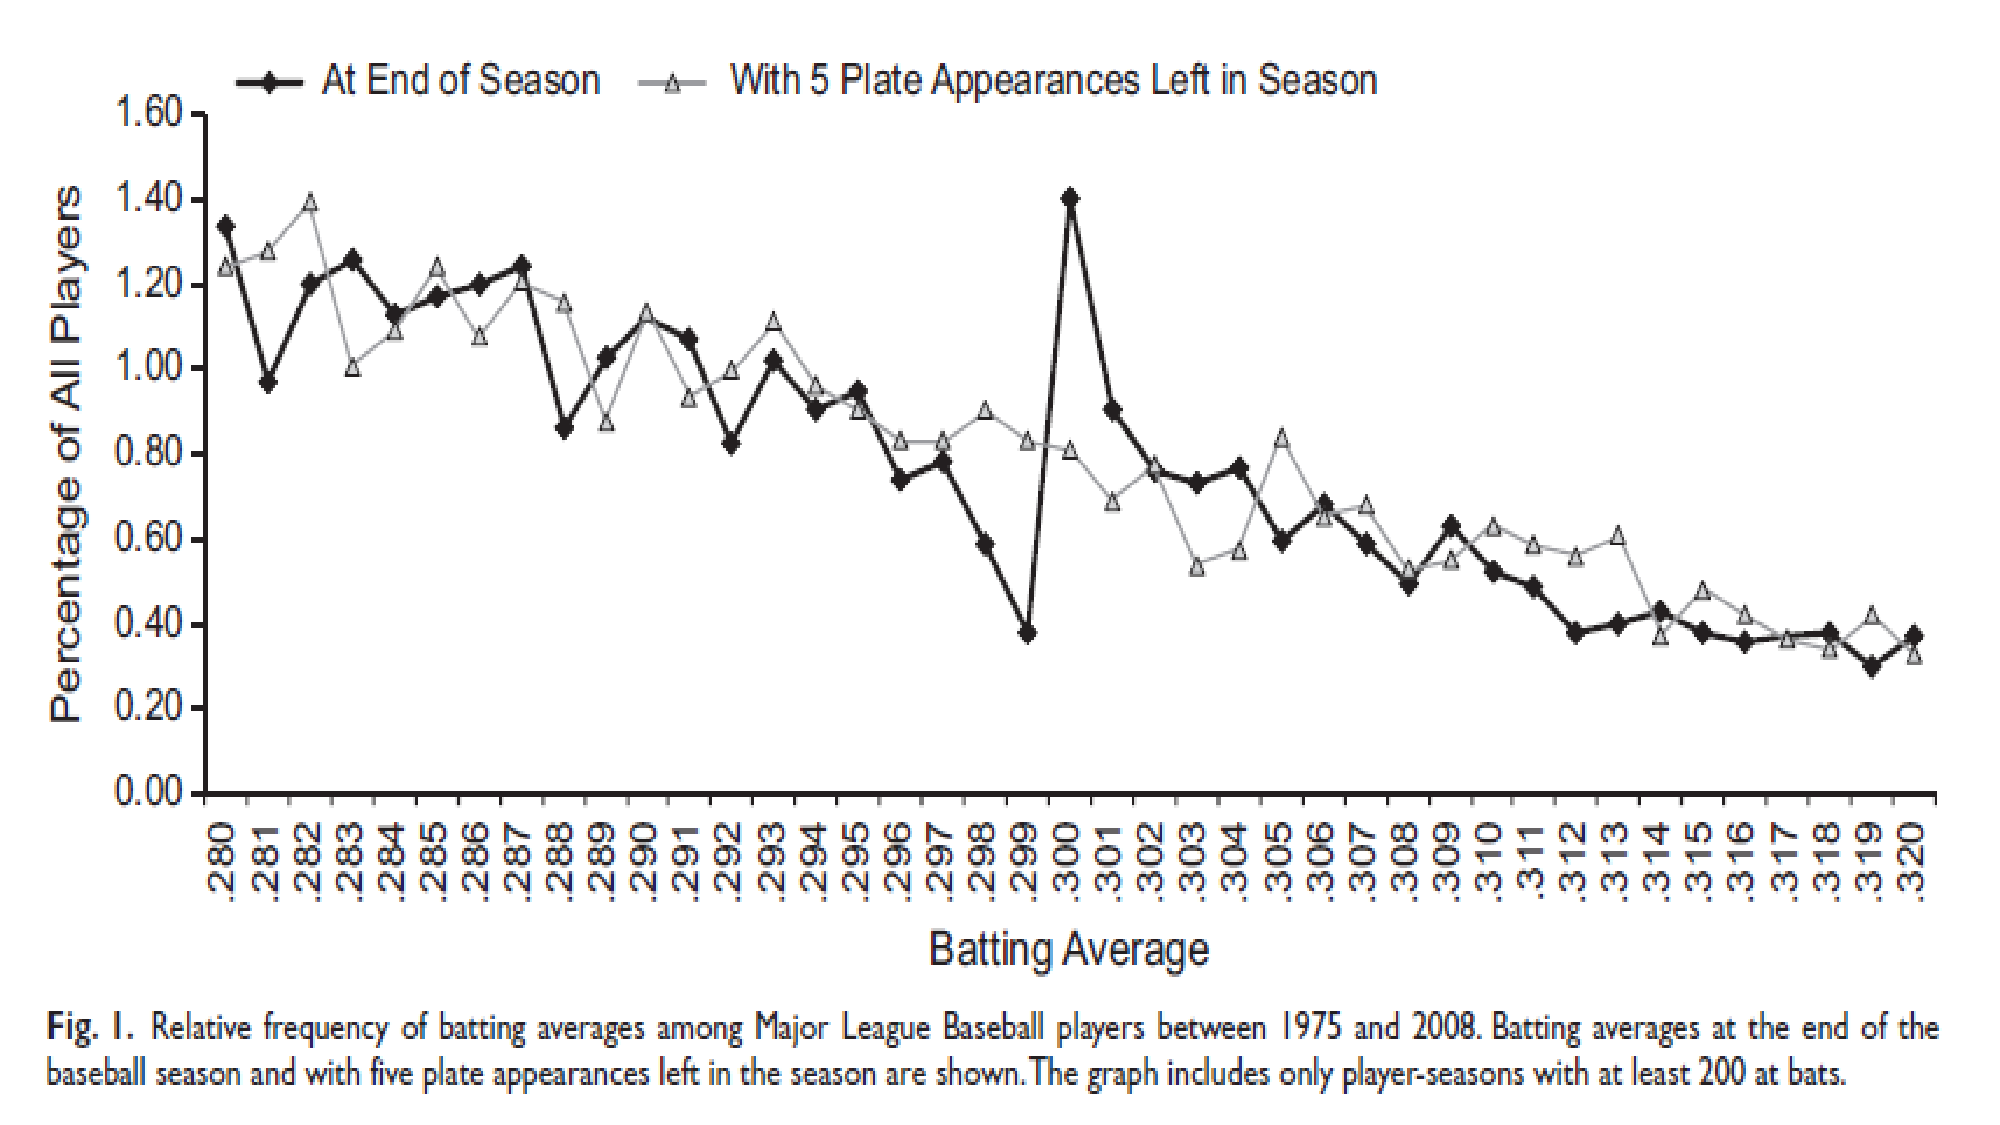
\includegraphics[width=12cm,height=5.25cm]{Pope_Simonsohn_F1.pdf}

\end{center}

 \begin{itemize}
 
 \item Players with .298 or .299 (0.97 \%) $<$ with .300 or .301 (2.30 \%), $Z=7.35$, $p<.001$.
 
 \item Control distribution : when 5 plate appearances left in the season.
 

 \end{itemize}

\end{frame}

\begin{frame}

\begin{center}

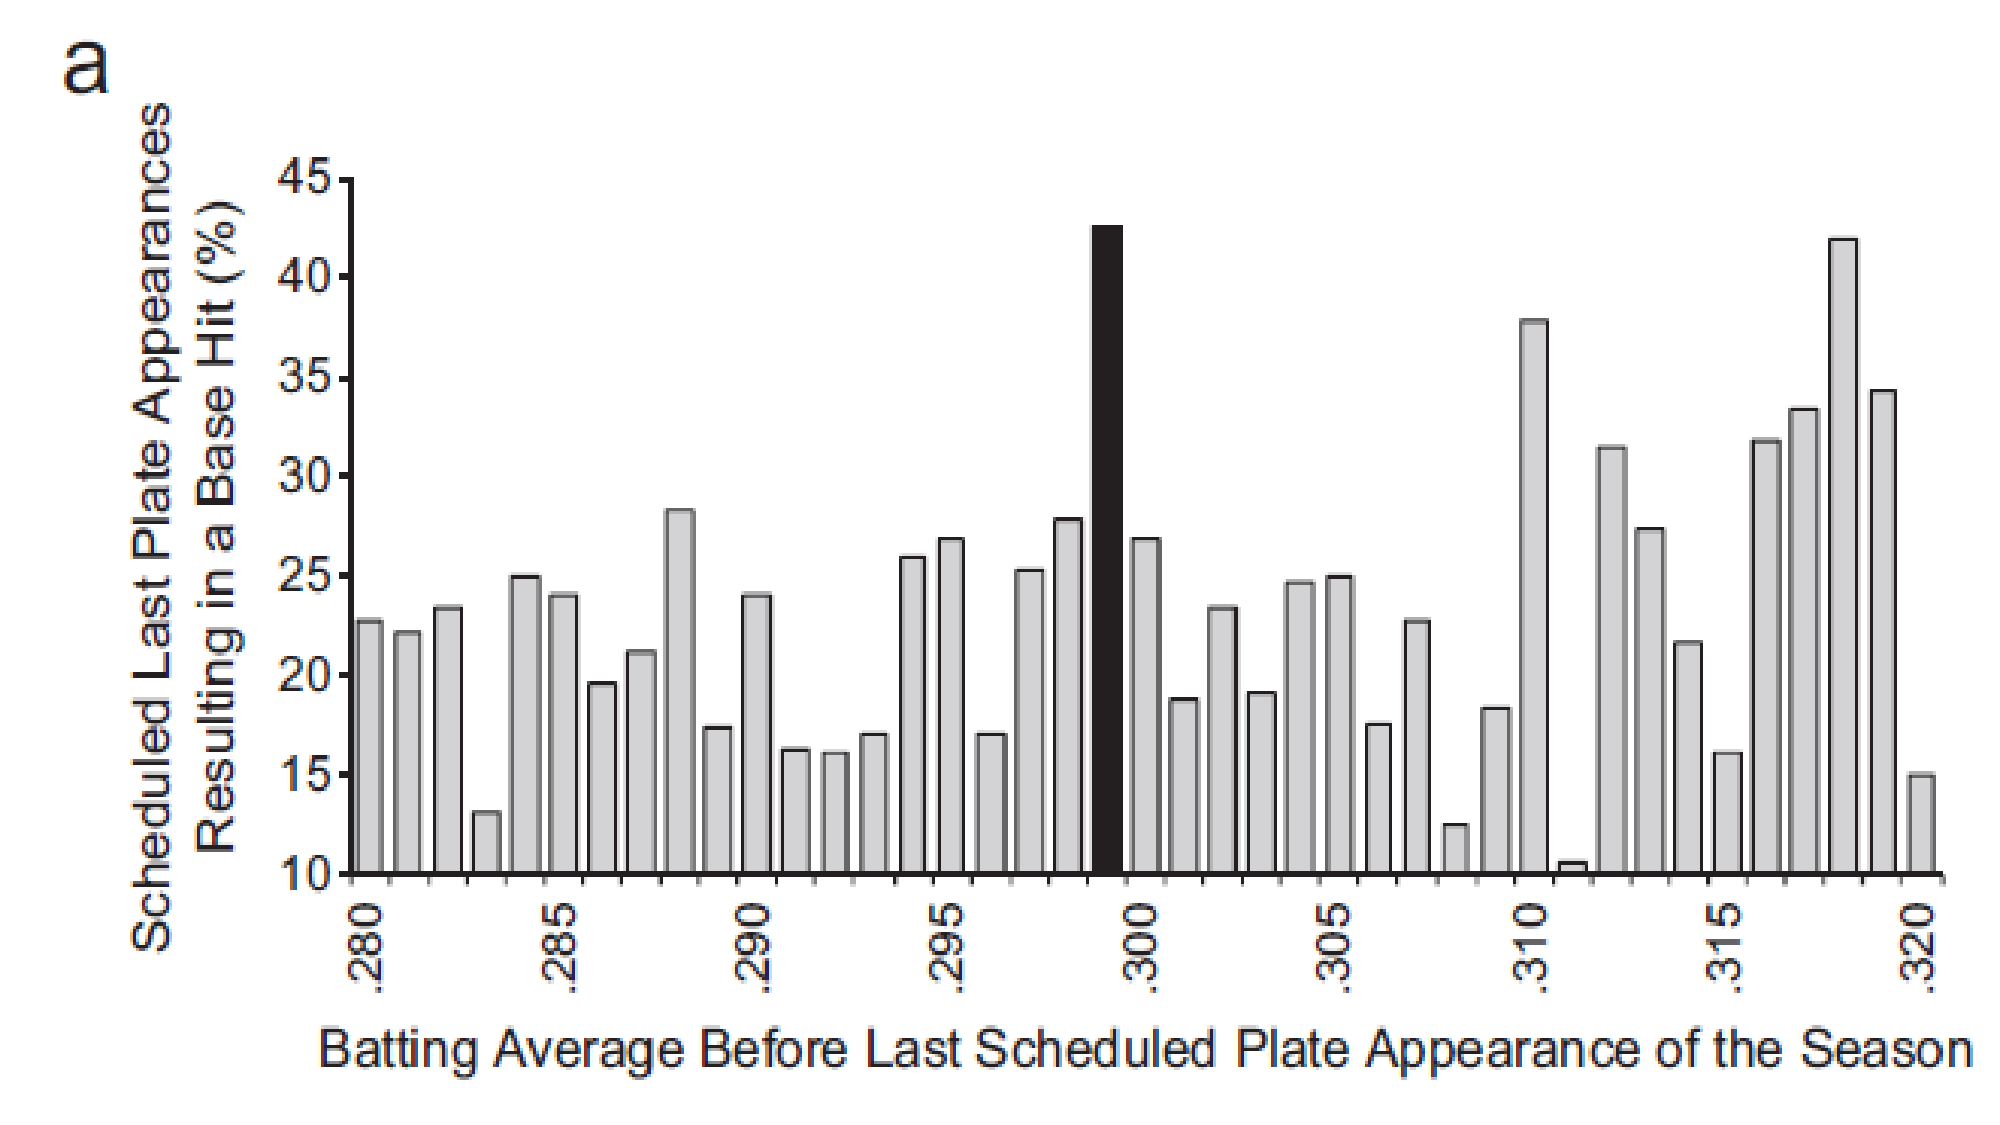
\includegraphics[width=10cm,height=5.75cm]{Pope_Simonsohn_F2A.pdf}

\end{center}

 \begin{itemize}
 
 \item Players with AVG of .299 was likely to get a base hit(43\%) than overall(22.8\%) at their last PA.
 
 $Z=3.62 , p <.001$.
 
 \end{itemize}

\end{frame}

\begin{frame}

\begin{center}

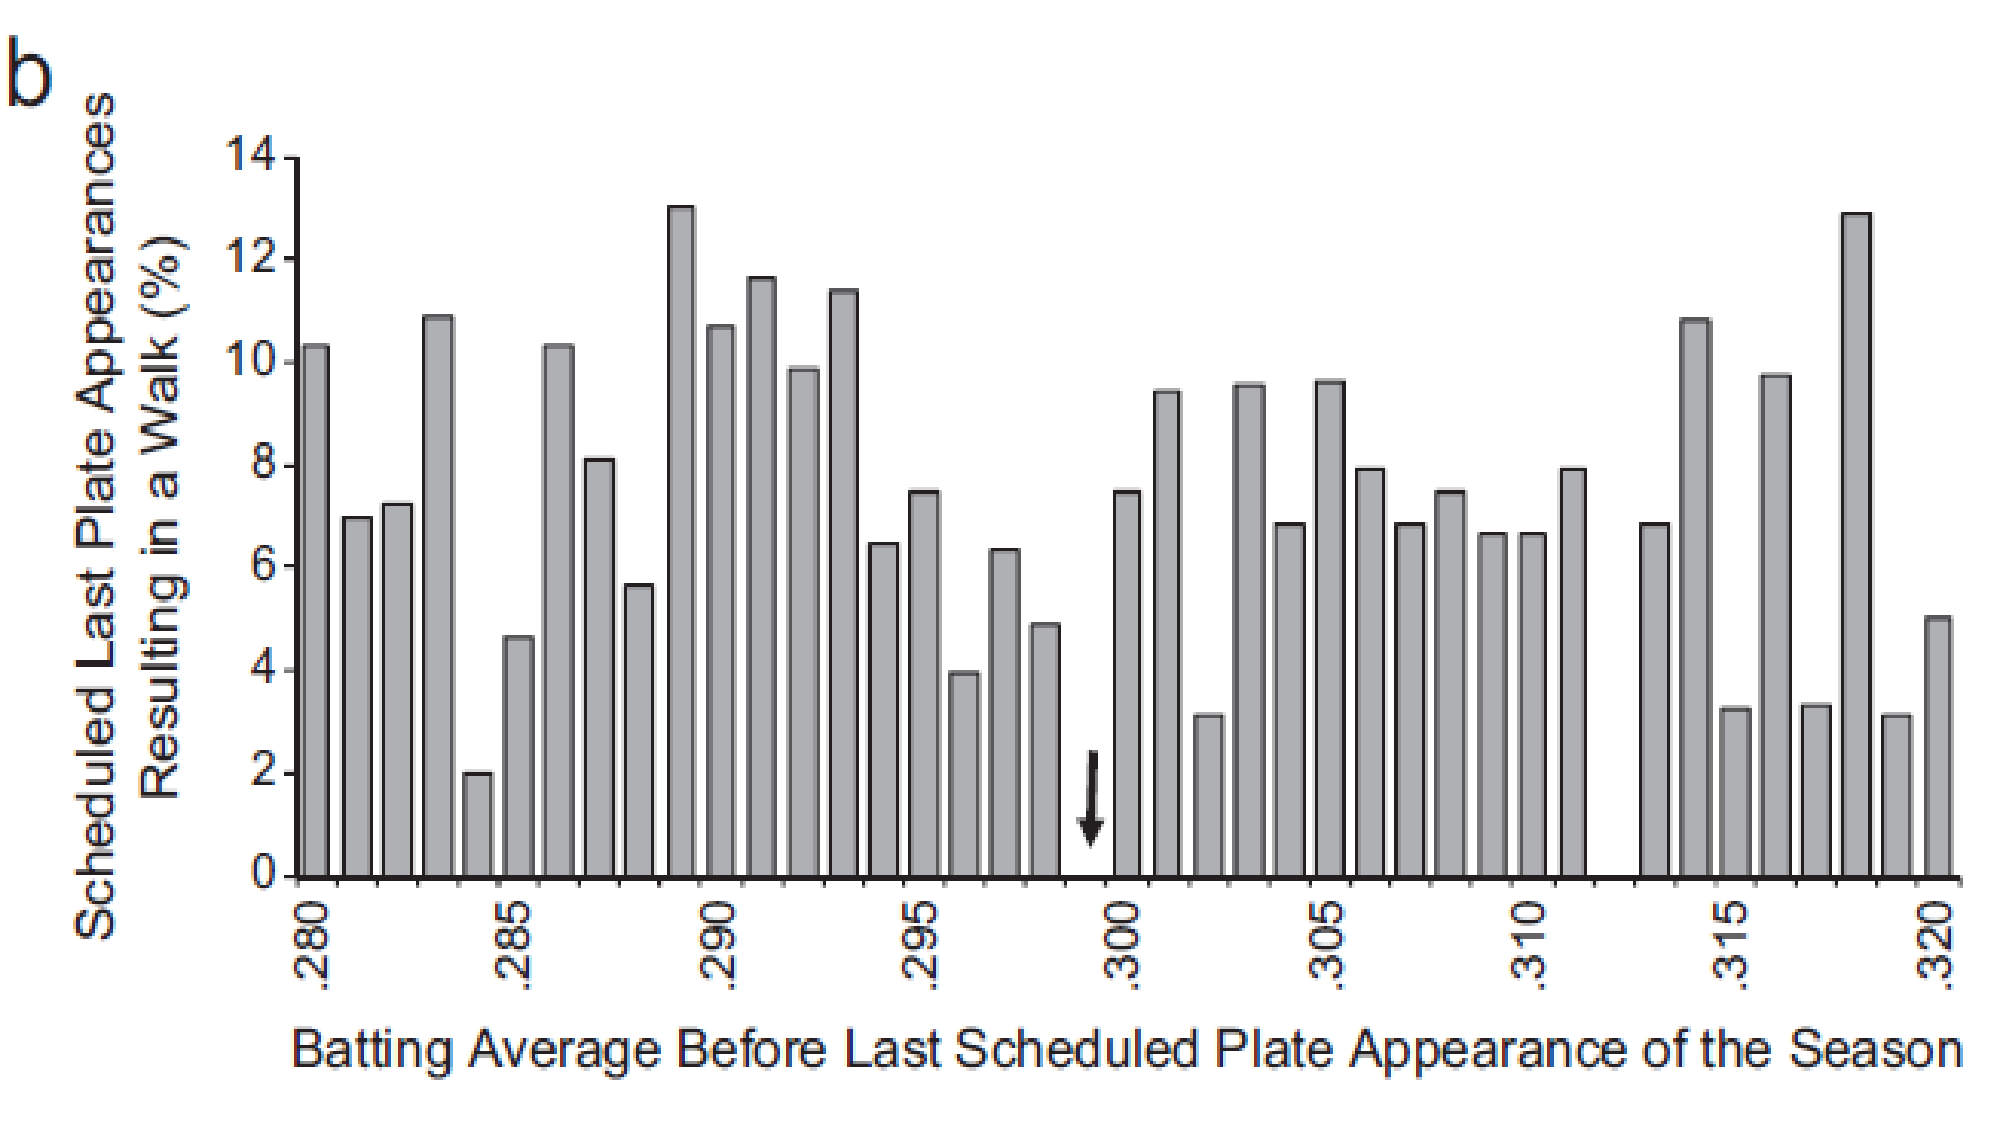
\includegraphics[width=10cm,height=5.75cm]{Pope_Simonsohn_F2B.pdf}

\end{center}

 \begin{itemize}
 
 \item .298 or .299 players tend to walk (四球) than .300 or .301 players.
 
 $Z=2.14$, $p=.032$.
 
 \end{itemize}

\end{frame}

\begin{frame}

\begin{center}

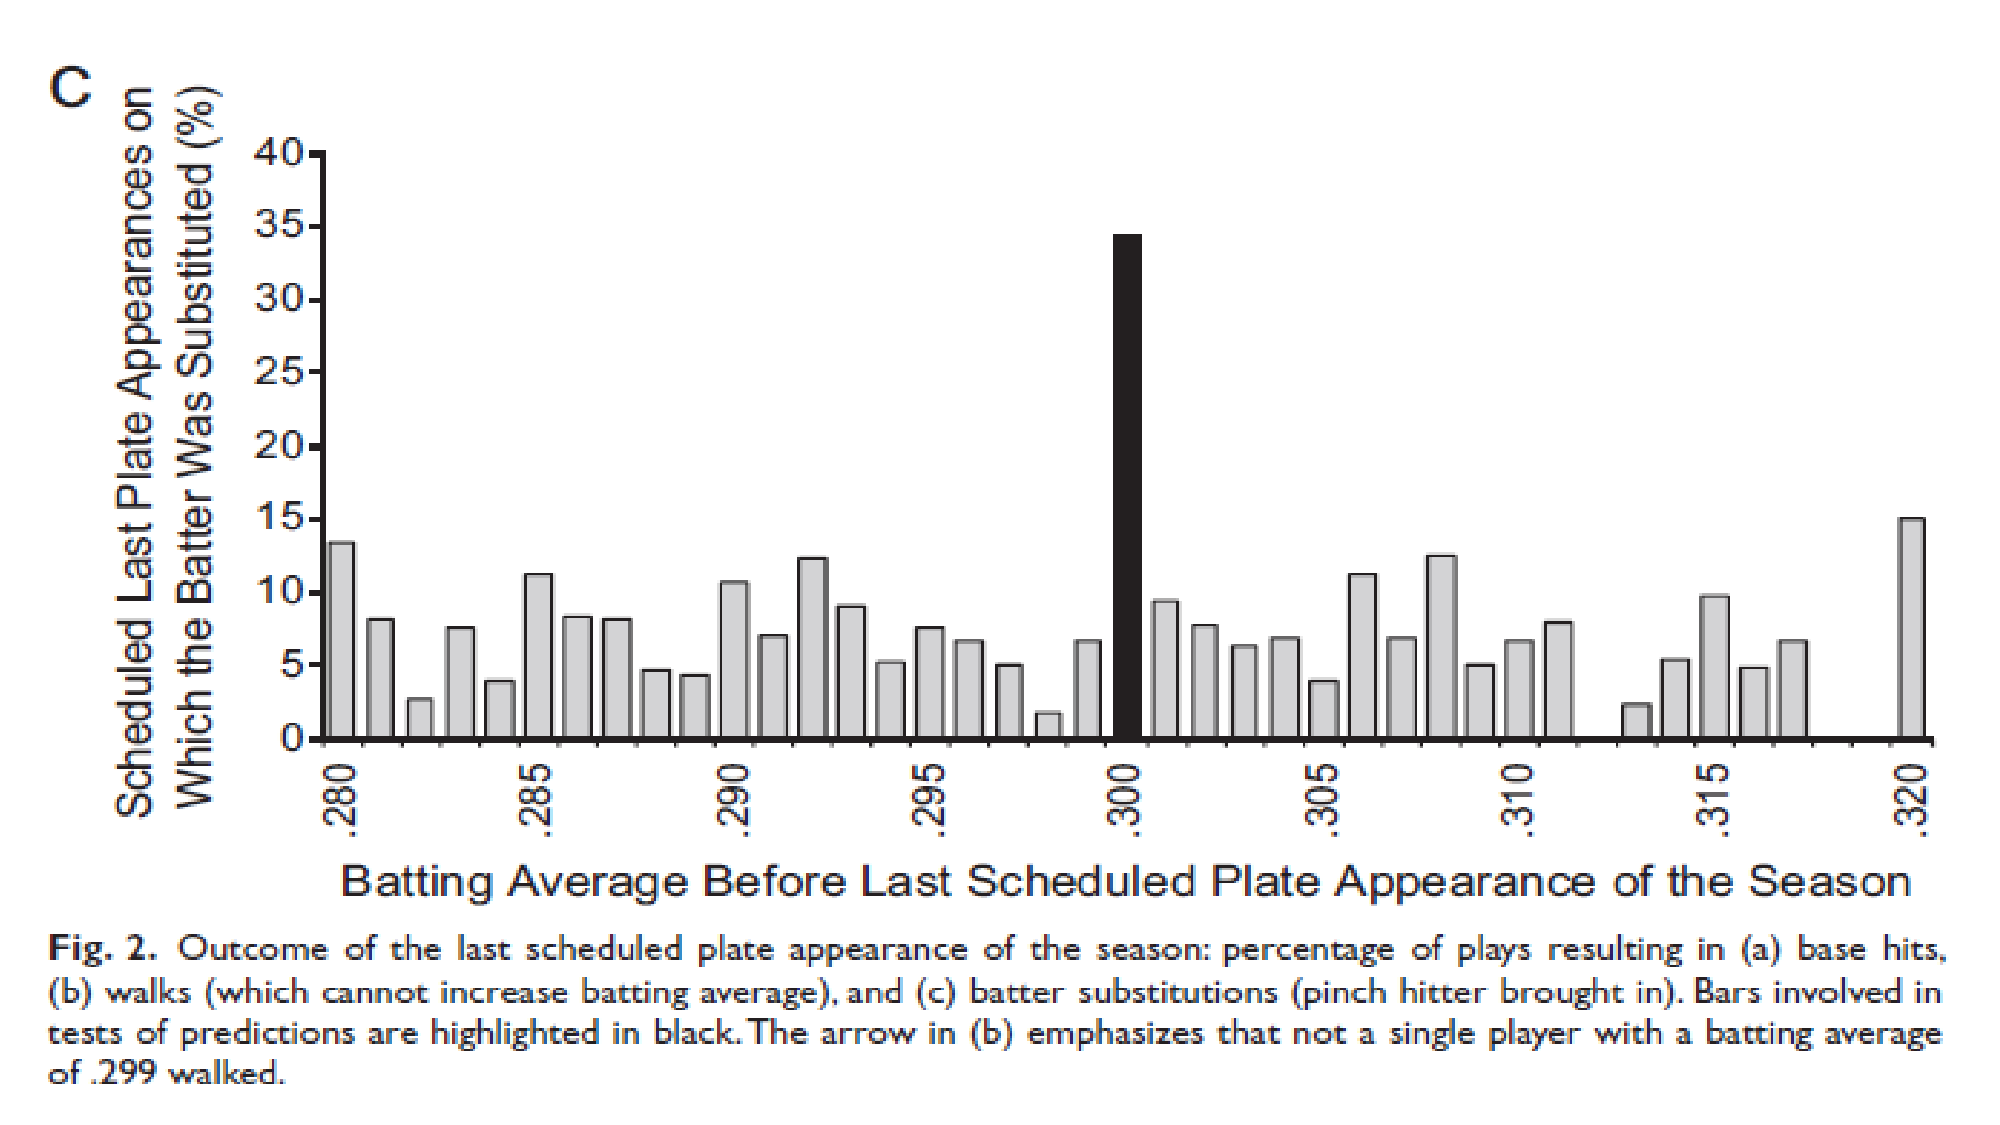
\includegraphics[width=9cm,height=5.75cm]{Pope_Simonsohn_F2C.pdf}

\end{center}

 \begin{itemize}
 
 \item If his AVG is just above .300, then he might end the season earlier by being substituted.
 
 $Z=8.29$ and $p<.001$.
 
 \end{itemize}

\end{frame}

\begin{frame}\frametitle{Pope \& Simonsohn}

 \begin{itemize}
 
 \item The behavior of baseball players proved the existence of the reference point of round numbers, such as batting average of .300.
 
 \item Limitations:
 
 There were only one relevant round number.
 
 Action to improve their performance took place on the last plate appearance.
 
 \end{itemize}

\end{frame}

\begin{frame}\frametitle{Hakes \& Sauer}

 \begin{itemize}
 \item \textit{``Moneyball Hypothesis''}
 
 : Michael Lewis's claim that the valuation of skills in MLB player's market was grossly inefficient.
 
 \item Members of the Society for American Baseball Research (In short, SABR) have studied that
 on-base percentage (OBP) plays more important role to consider the winning percentage than batting average.
 
 \end{itemize}

\end{frame}

\begin{frame}

\begin{center}

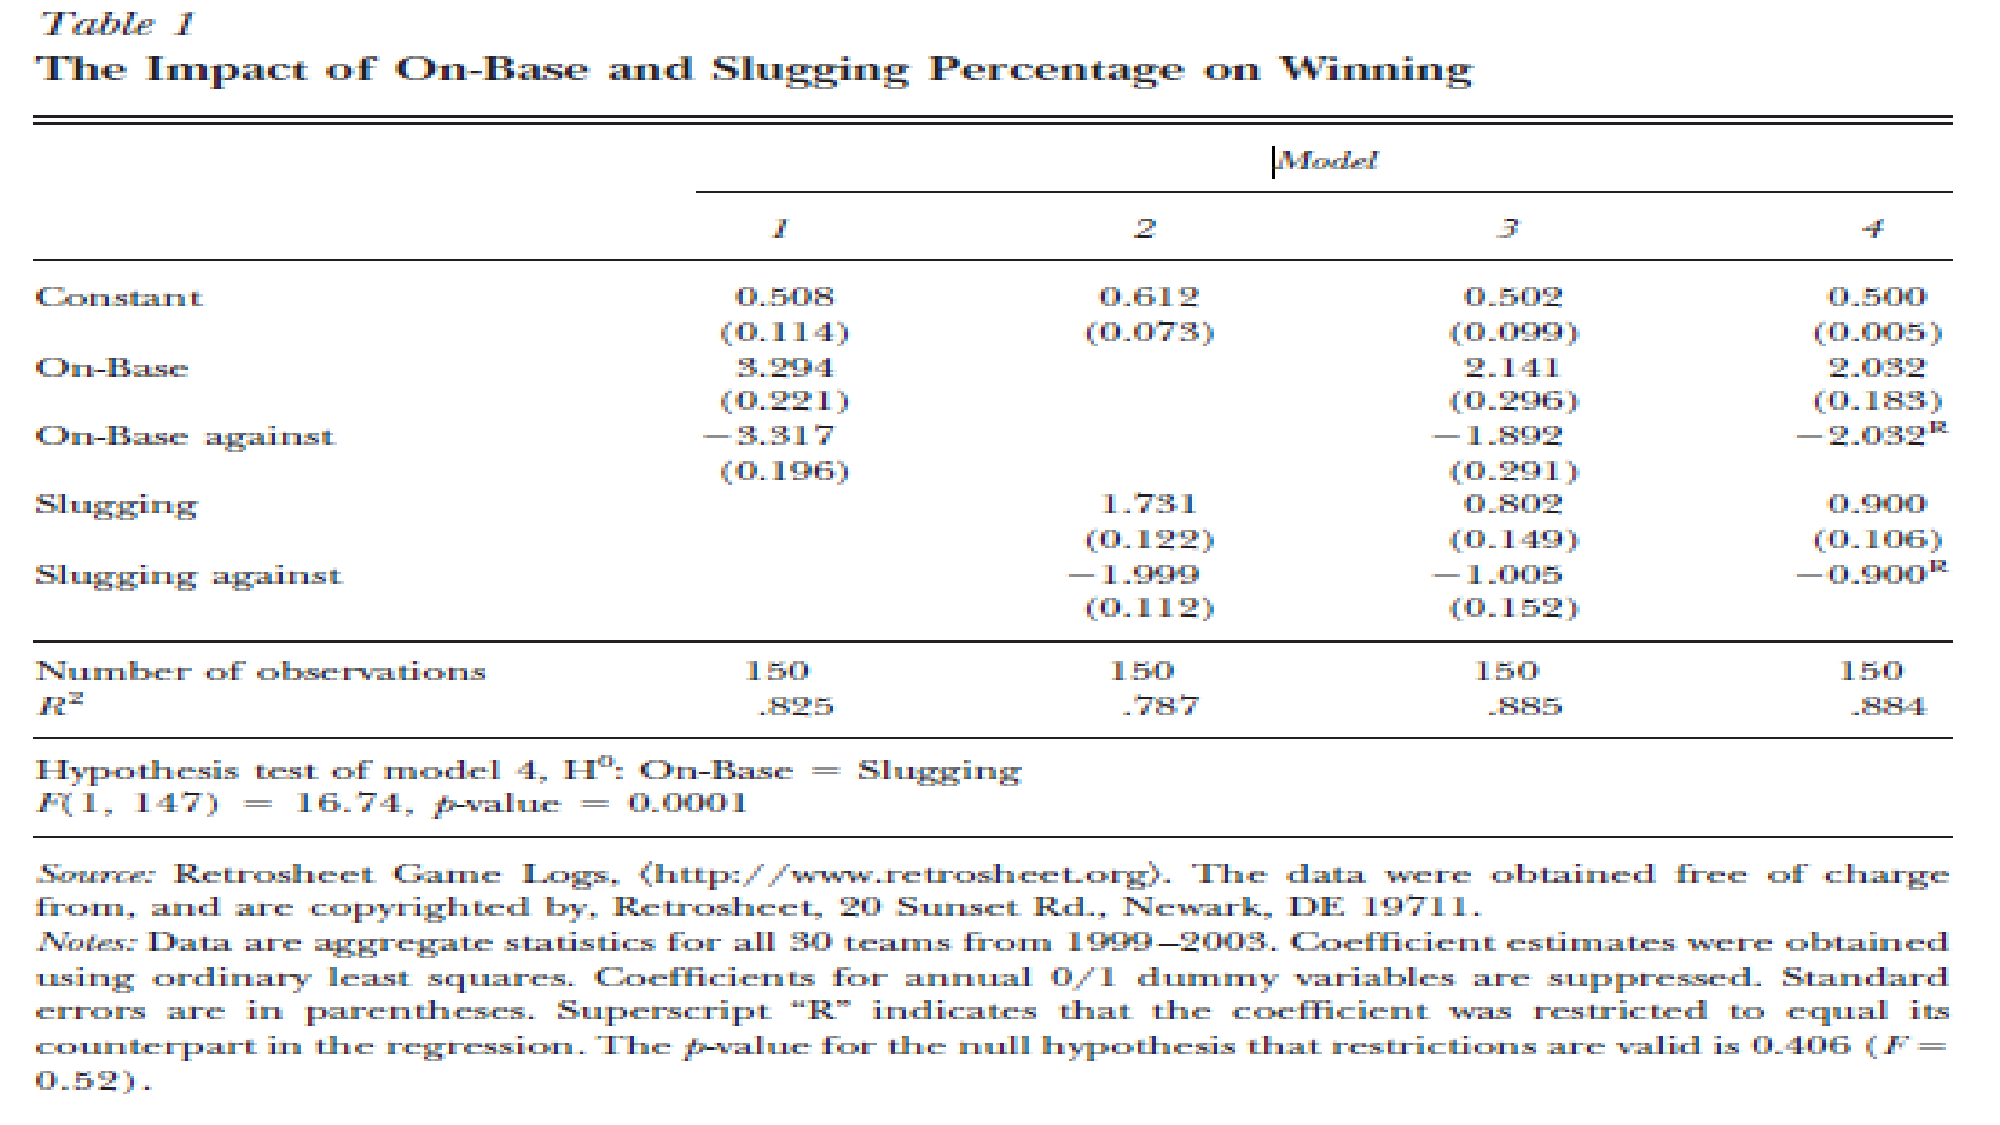
\includegraphics[width=9cm,height=7.75cm]{Hakes_Sauer_T1.pdf}

\end{center}

\end{frame}

\begin{frame}

\begin{center}

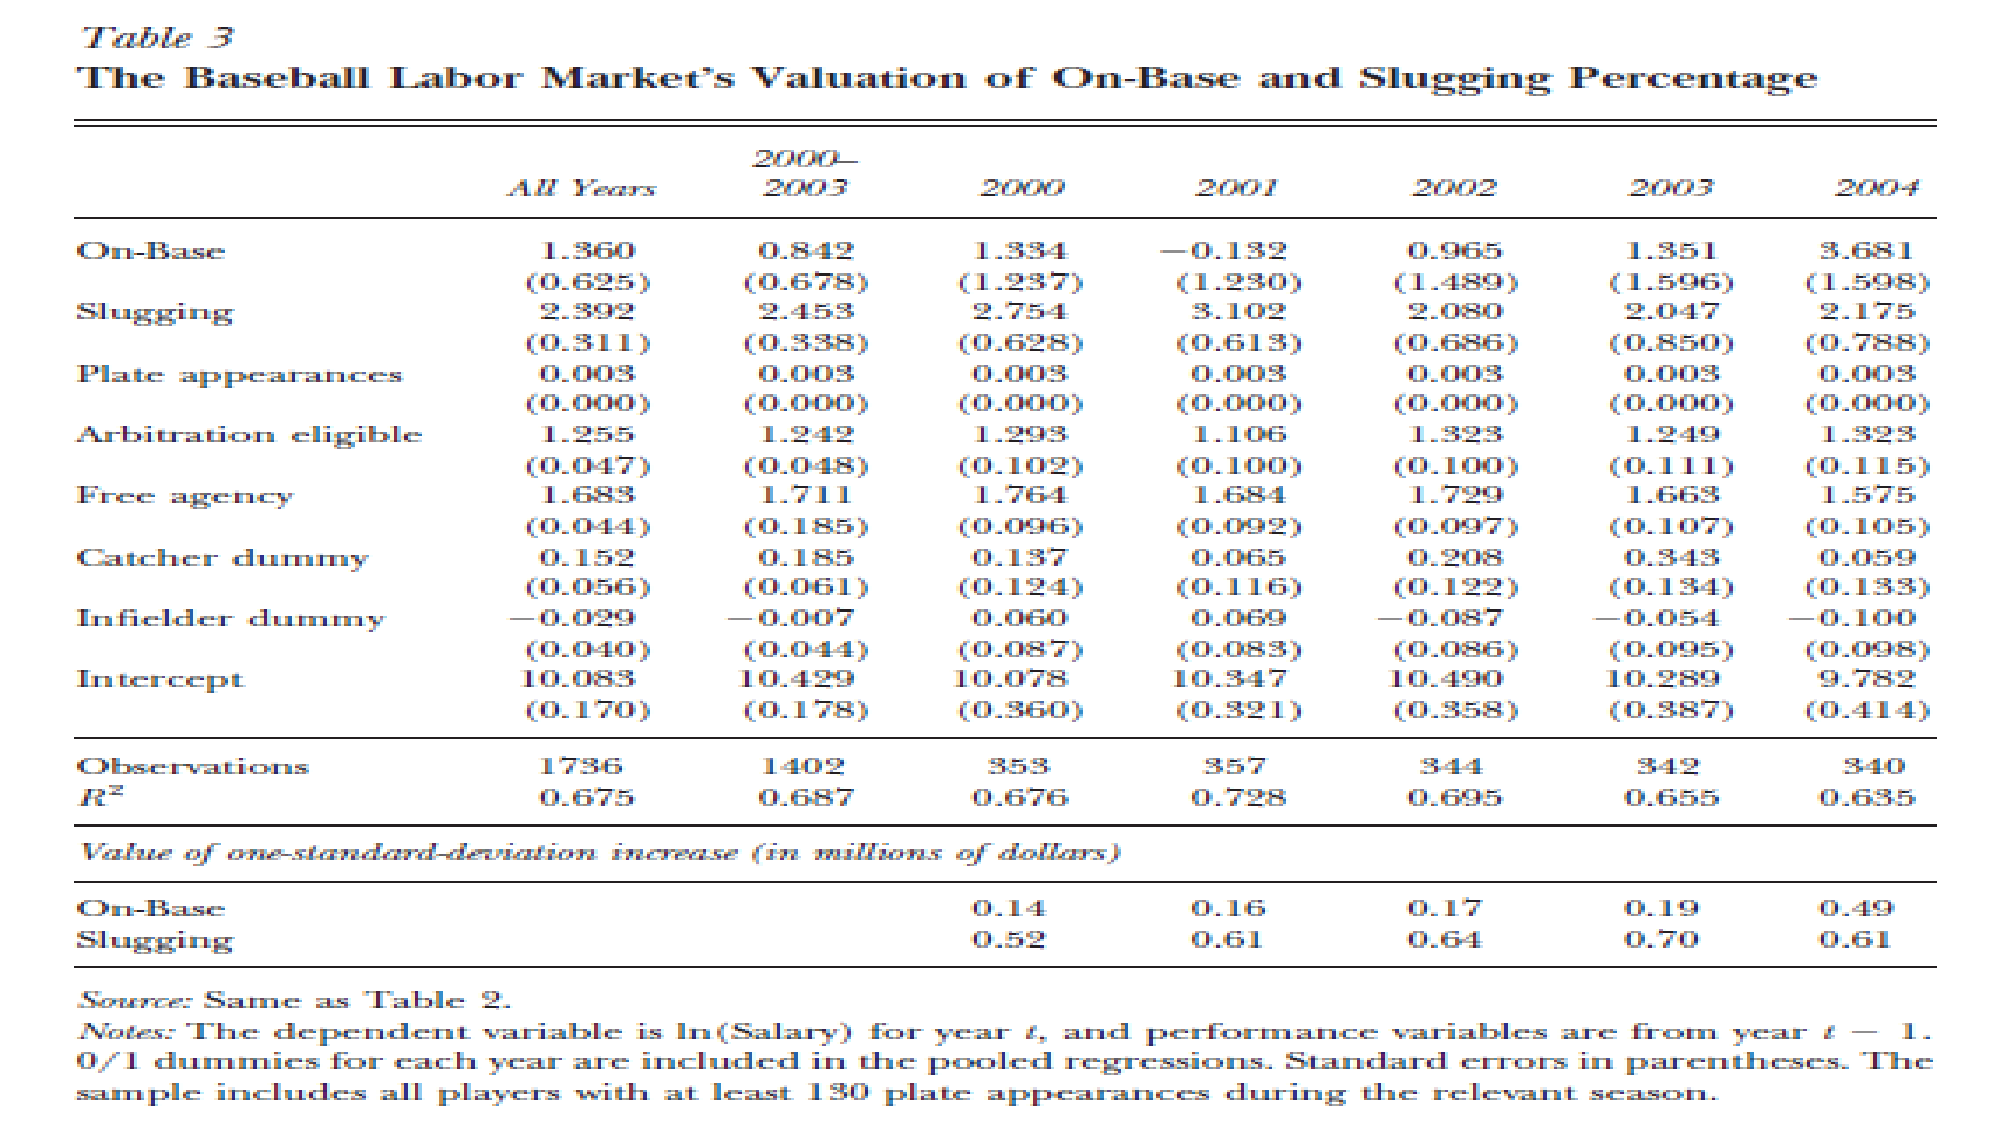
\includegraphics[width=9cm,height=7.75cm]{Hakes_Sauer_T3.pdf}

\end{center}

\end{frame}

\begin{frame}

\begin{center}

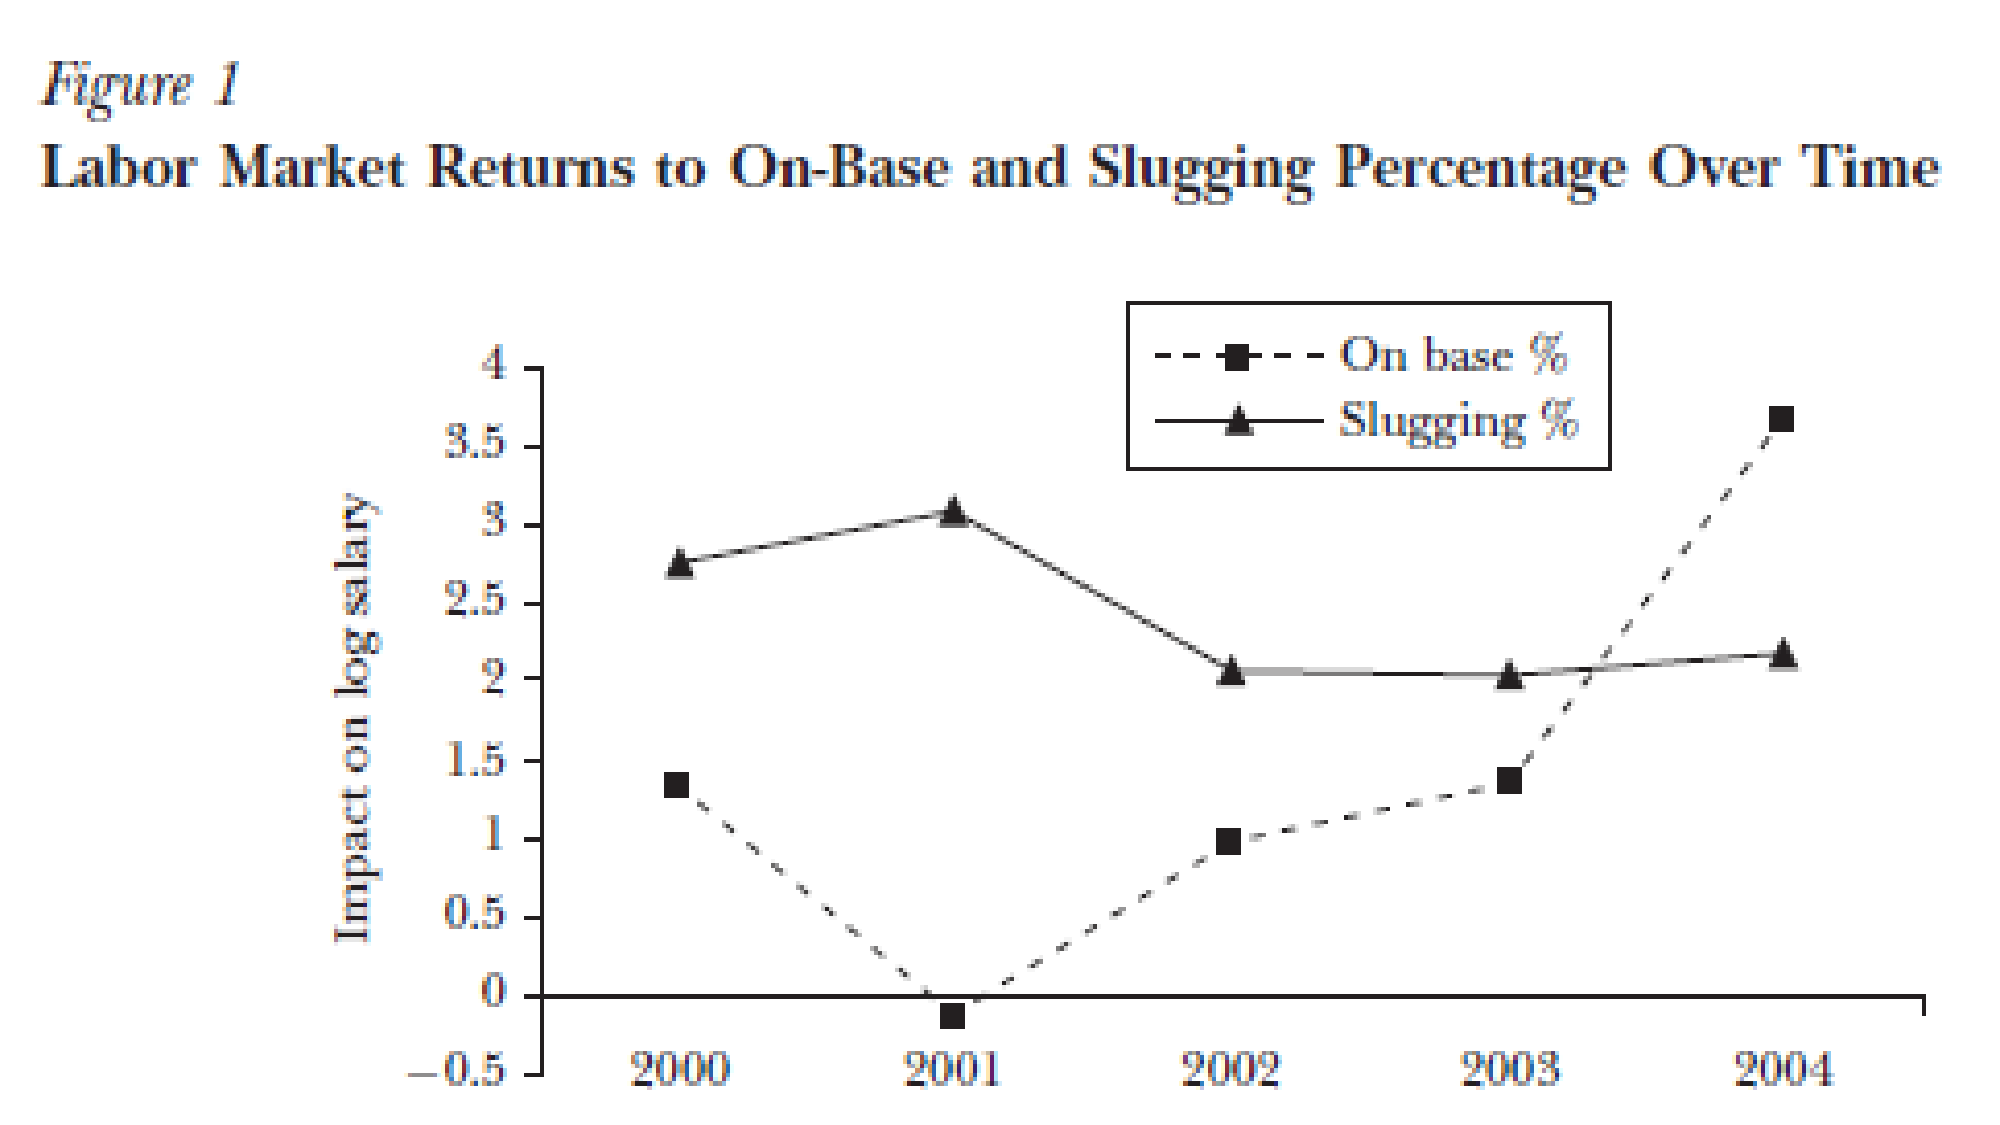
\includegraphics[width=11cm,height=5.75cm]{Hakes_Sauer_F1.pdf}

\end{center}

\end{frame}

\begin{frame}

\begin{center}

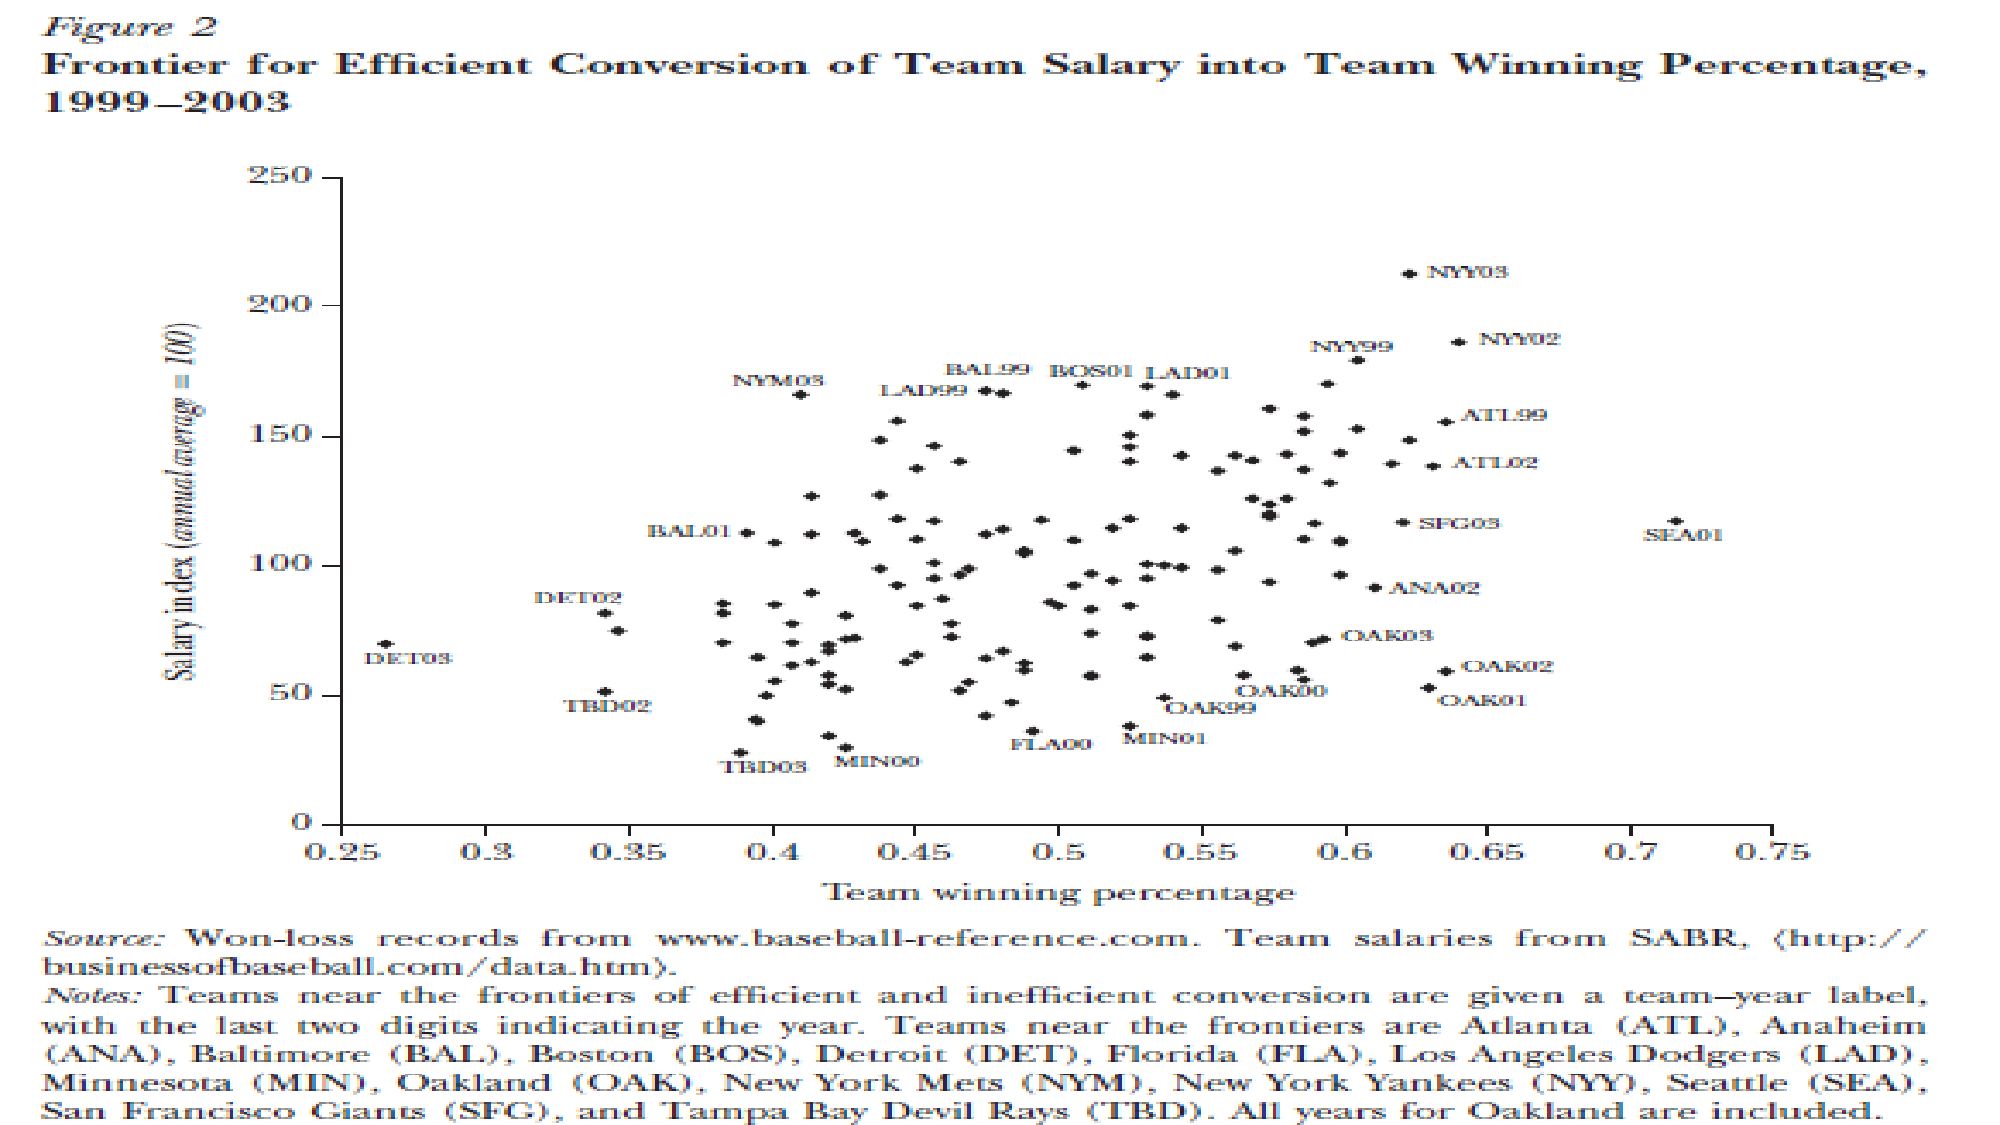
\includegraphics[width=10.5cm,height=8cm]{Hakes_Sauer_F2.pdf}

\end{center}

\end{frame}

\begin{frame}\frametitle{Extension}

 \begin{itemize}
 
 \item On-base percentage may be more important than batting average, when it comes to consider raising winning percentage, and it reflects players' effort in similar way to batting average.
 
 $\Rightarrow$ Round numbers in on-base percentage may act as reference point, as well as batting-average : .350 or .400.
 
 \end{itemize}

\end{frame}

\begin{frame}\frametitle{Data}

 \begin{itemize}
 
 \item Sortable team stats of Nippon Professional Baseball (NPB), from 2008 to 2017.
 
 : N=120
 
 \item Indexes : Win average (勝率 : WA), Runs (得点 : R) Runs allowed (失点 : RA), Batting average (AVG),
 On-base percentage (出塁率 : OBP) Slugging percentage(長打率 : SLG), OPS (OBP + SLG).
 
 \end{itemize}

\end{frame}

\begin{frame}\frametitle{Model}

 \begin{itemize}
 
 \item Confirm that also in NPB, OBP contributes better to the Win Average than AVG or SLG.
 
 Applying OLS,
 
 \[\textit{WA}_i = \beta \mathbf{X}_i + \textit{RA}_i + u_i \]
 
 \[\textit{R}_i = \gamma \mathbf{X}_i + v_i \]
  
  \begin{align*}
  \textit{WA}_i &: \text{Win average of team } i \\
  \textit{R}_i &: \text{Runs of team } i \\
  \mathbf{X}_i &: \text{OBP, SLG and AVG of the team } i
  \end{align*}
 
 \end{itemize}

\end{frame}






\end{document}